\section{Overview on Urban Heat}
	One of the United Nations’ ``17 Sustainable Development Goals'' is Sustainable Development Goal 11 (SDG 11): ``Sustainable Cities and Communities.'' 
	SDG 11 is a goal to make human settlements inclusive, safe, resilient, and sustainable (\cite{UN2015}).
	
	In line with SDG 11, one big problem that cities are facing is the ``urban heat island.'' 
	This problem refers to the phenomenon where urban areas have higher temperatures compared to rural areas (\cite{Khan2021}).
	This problem is further exacerbated by climate change, and can cause discomfort (\cite{Bhati2018}), worsen ambient air quality, and increase morbidity and mortality (\cite {Khan2021}).
	
	There are several factors that can contribute to urban heat islands.
	One factor is anthropogenic heat, which is heat created by human activies.
	Examples of anthropogenic heat include heat from vehicles and air conditioners (\cite{Kim2021}).
	Another factor is the thermal properties of buildings in urban areas. 
	Some materials used in infrastructures tend to have high heat absorption (\cite{Kim2021}). 
	Another factor is the morphology, or the shape, of the urban area.
	Radiation and warm air can be trapped inbetween buildings, for example (\cite{Wang2023}). 
	Other factors can be climatological or socioeconomic in nature (\cite{Khan2021}).

\section{Summary of Studies on Urban Heat}	
	\subsection{North America and Europe}
		\textcite{Fallmann2016} modeled how mitigation measures for urban heat islands affected air quality in Stuttgart, Germany using WRF-Chem and a multi-layer canopy model. Findings include: 
			peak ozone concentration increasing for white roofs, 
			increase of primary pollutants due to reduced vertical mixing; and 
			decreasing average ozone concentration for urban greening and white roofs.
		
		\textcite{Karlicky2018} evaluated the impact of urban surfaces on the climate of Berlin, Munich, and Prague.
		Its simulation domain can be seen in Figure \ref{fig:rrl-karlicky2018-domain}.
		The authors used two models: the Weather Research and Forecasting (WRF) model and Regional Climate Model (RegCM).
		An average of $\qtyrange{2}{3}{\degreeCelsius}$ increase in temperature due to the urban heat island effect was reported.
		Graphs of the averaged daily temperature cycles of Prague can be seen in Figure \ref{fig:rrl-karlicky2018-dailytemps}.
		They also reported that urban effects could decrease concentration of primary pollutants.
		Wind speed due to urban effects were highly dependent on the model and parametrizations used, though all of them were able to replicate the urban heat islands.
		
		\begin{figure}
			\centering
			\subfloat[
				Position of the model domain with model topography in \qty{10}{km} resolution (\unit{m}).
				Grid boxes with dominant urban land use are marked in red colour.
				From the bottom, the cities of Munich, Prague and Berlin are marked.
			]{
				\label{fig:rrl-karlicky2018-domain}
				\centering
				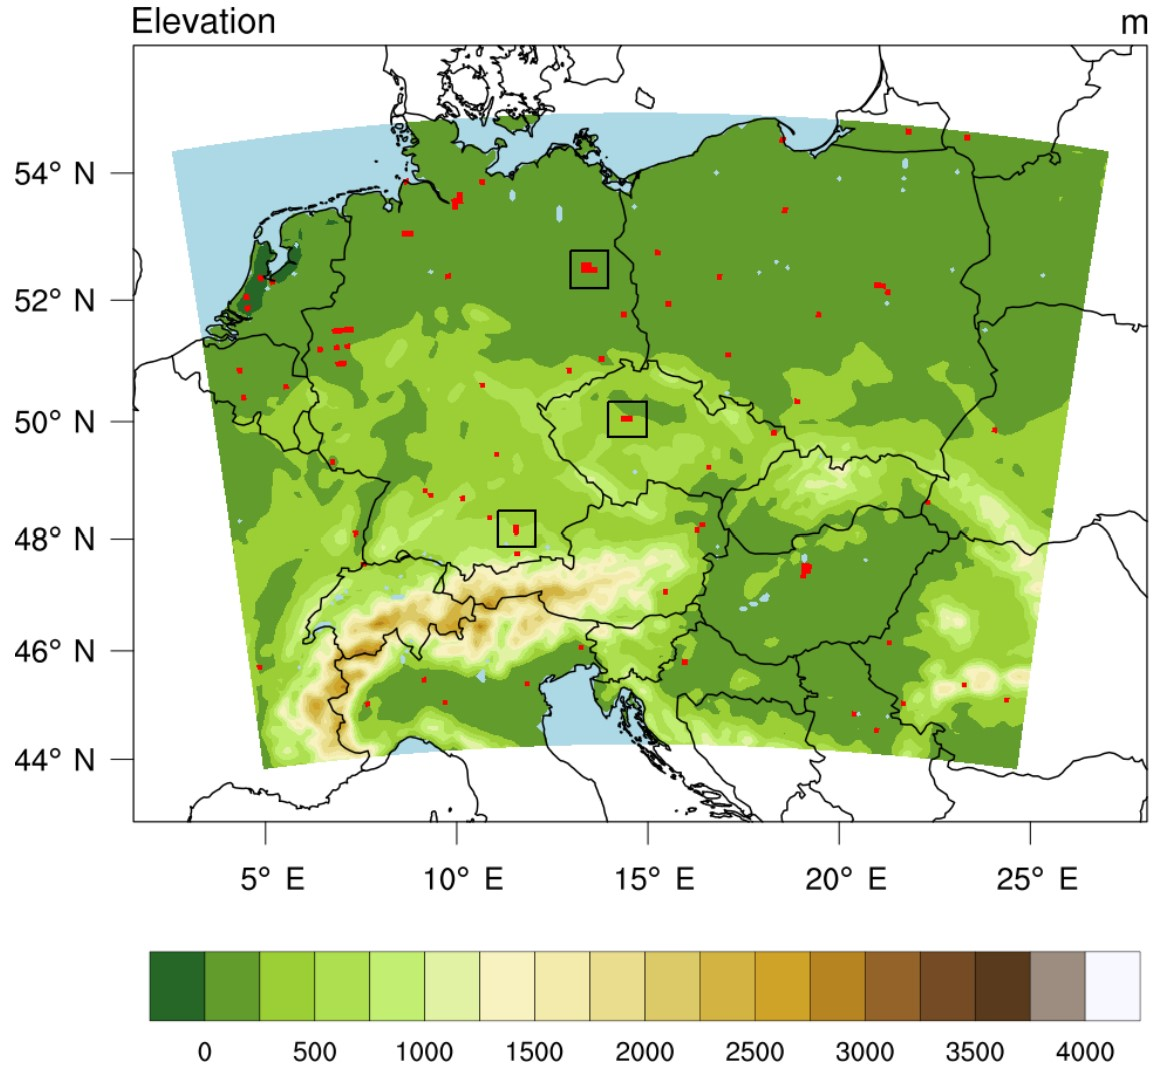
\includegraphics[width=0.45\linewidth]{rrl-karlicky2018-domain}
			}
			%nospace
			\hfill
			\subfloat[
				Averaged daily temperature cycles (\unit{\degreeCelsius}) in the Prague city centre (red), in its surroundings (green) and those simulated with the urban surface removed (black).
			]{
				\label{fig:rrl-karlicky2018-dailytemps}
				\centering
				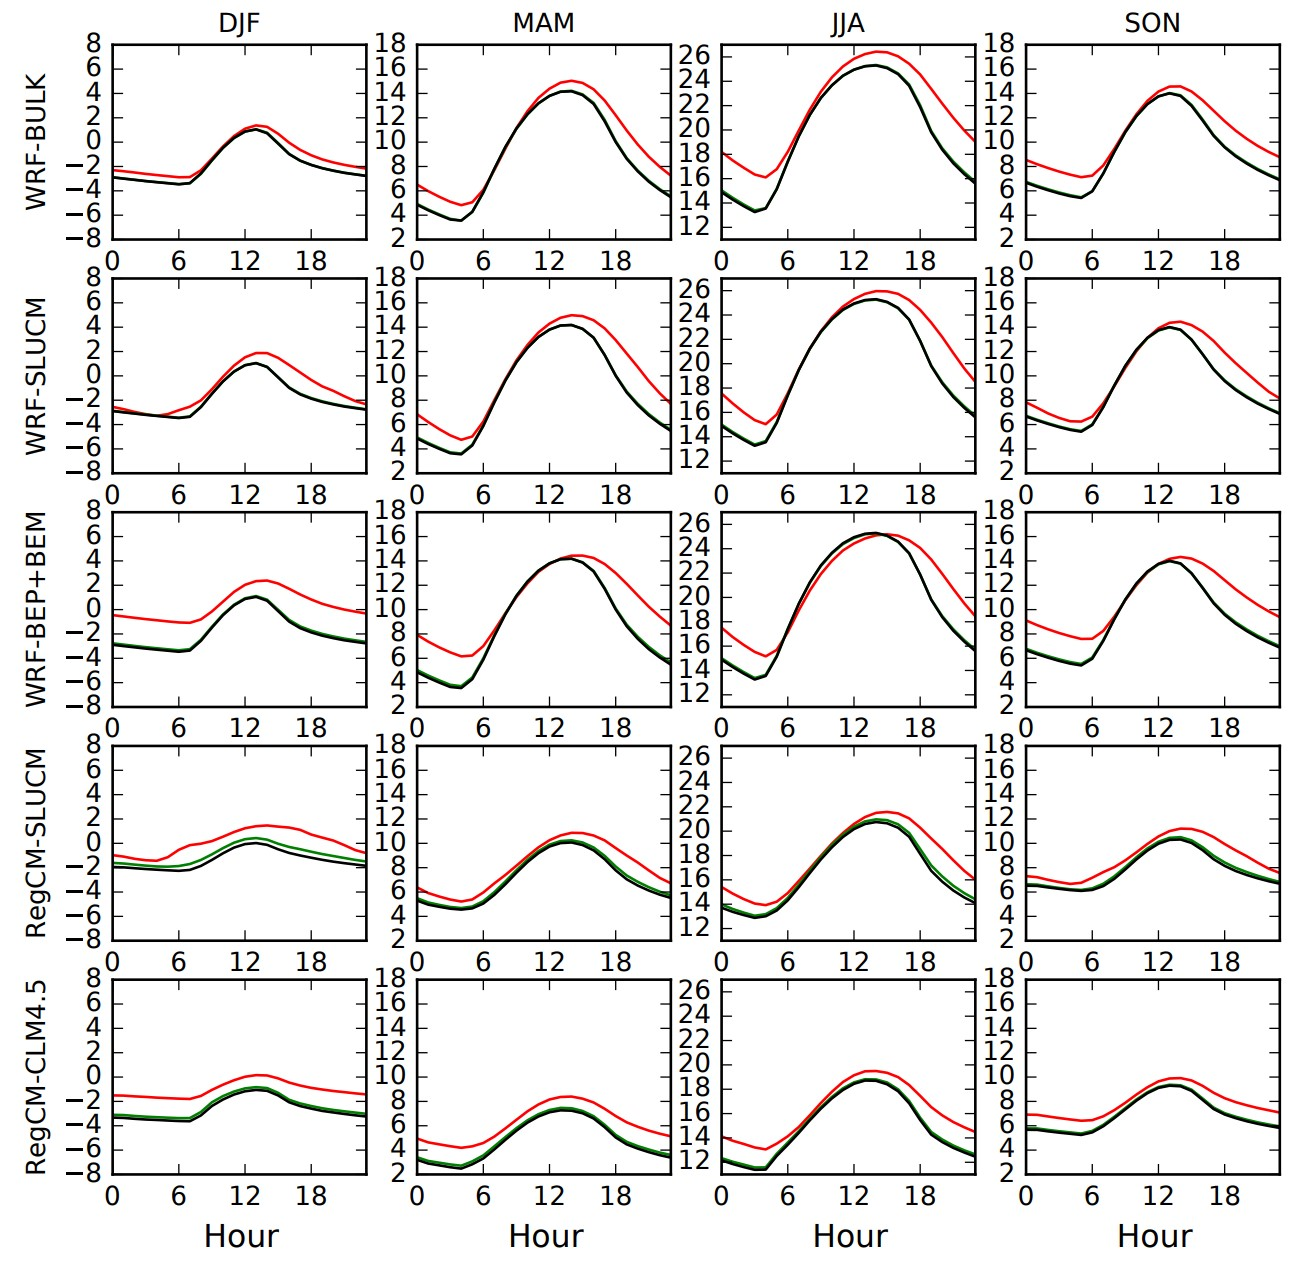
\includegraphics[width=0.45\linewidth]{rrl-karlicky2018-dailytemps}
			}
			
			\caption{Figures from \textcite{Karlicky2018}.}
			\label{fig:rrl-karlicky2018}
		\end{figure}
		
		\textcite{Ziter2019} evaluated the effectiveness of tree canopy cover as a mitigation strategy for urban heat.
		The authors attached sensors and a GPS device to a bike and rode around Madison, Winsconsin, USA.
		Using generalized additive models in R, they found that enough canopy cover can significantly help with cooling cities, 
			with results showing about a $\qty{1}{\degreeCelsius}$ drop in temperature.
		The researchers note that a $\qty{40}{\percent}$ canopy cover is needed in order to get the most cooling.
		
		\textcite{Hsu2021} investigated the distribution of urban heat across the US demographic. 
		They compared the land surface temperature from remote sensing with data from the US Census.
		The mean surface urban heat intensity was found to be $\qty{2.2}{\degreeCelsius}$.
		The average person-of-color was found to live in areas of higher urban heat intensity than white people.
		Similarly, people below the poverty line lived in areas of higher urban heat intensity compared to those who were twice above the poverty line.
		
		\textcite{Huszar2018} used RegCM to study the impact of urbanization on aerosols concentrations in Prague, the Czech Republic.
		They found that urban heat effects caused a $\qtyrange{2}{3}{K}$ increase in temperature, and a wind speed reduction of about $\qty{1}{m/s}$.
		They also found that secondary inorganic aerosols (such as nitrates) were the main contributor to the increase in temperature compared to other contributors.
		
				
	\subsection{Asia}
		\textcite{Yuan2020} conducted a computational parametric study in order to evaluate the impact of urbanization in Singapore.
		Using Computational Fluid Dynamics, they examined how anthropogenic heat disperses given the city's urban morphology.
		The authors discovered that heat is hard to disperse if there is a lack of incoming wind.
		Based on the findings, the authors created a practical modeling tool in order to help with urban planning. 
		The Geographic Information System-based tool estimates how much impact anthropogenic heat has on the city's ambient temperature.
		
		\textcite{Gao2019} explored how effective different strategies are in mitigating the surface urban heat island in Wuhan China.
		Using the offline urbanized High-Resolution Land Data Assimilation System (u-HRLDAS), they showed that the best mitigation strategy for daytime urban heat islands is using green roofs and cool roofs.
		In their follow-up study (\cite{Gao2020}), the authors compared mitigation strategies in Wuhan, China to Xi'an, China.
		They found that all the mitigation strategies they considered were more effective for Xi'an than it was for Wuhan. 
		The authors explain that this is due to the differences in regional climate.
		
		\textcite{Wang2019} presented their preliminary findings on their modeling of Kuala Lumpur, Malaysia using ADMS-Urban.
		The authors verified their findings with landsat images, though their original plan was to use data from local meteorological stations.
		Wind speed depends on the time of day, but is shown to have a general inverse relationship with the intensity of the urban heat island effect.
		The study reported an urban heat island intensity of $\qty{8}{\degreeCelsius}$.
		The study did not take into account anthropogenic heat.
		
		\textcite{Bhati2018} studied the urban heat island effect in Delhi, India using WRF and four different data sets on land use/land cover.
		They report that urban areas were $\qtyrange{1.5}{2}{\degreeCelsius}$ hotter than rural areas, leading to a heat index change of $\qtyrange{2.0}{2.5}{\degreeCelsius}$.
		This hotter heat index can lead to more thermal discomfort.

	\subsection{The Philippines}
		\textcite{AlmadronesReyes2022} used remote sensing technology to examine how land use has changed in Metro Manila from 2001 to 2019. 
		They also examined the relationship between green spaces and temperature. 
		Their results show a decrease in normalized difference vegetation index, 
			as well as a $\qty{4}{\degreeCelsius}$ difference from 2001 to 2019.
		Maps of their findings can be seen in Figure \ref{fig:rrl-almadronesreyes2022-mm}.
		
		\begin{figure}
			\centering
			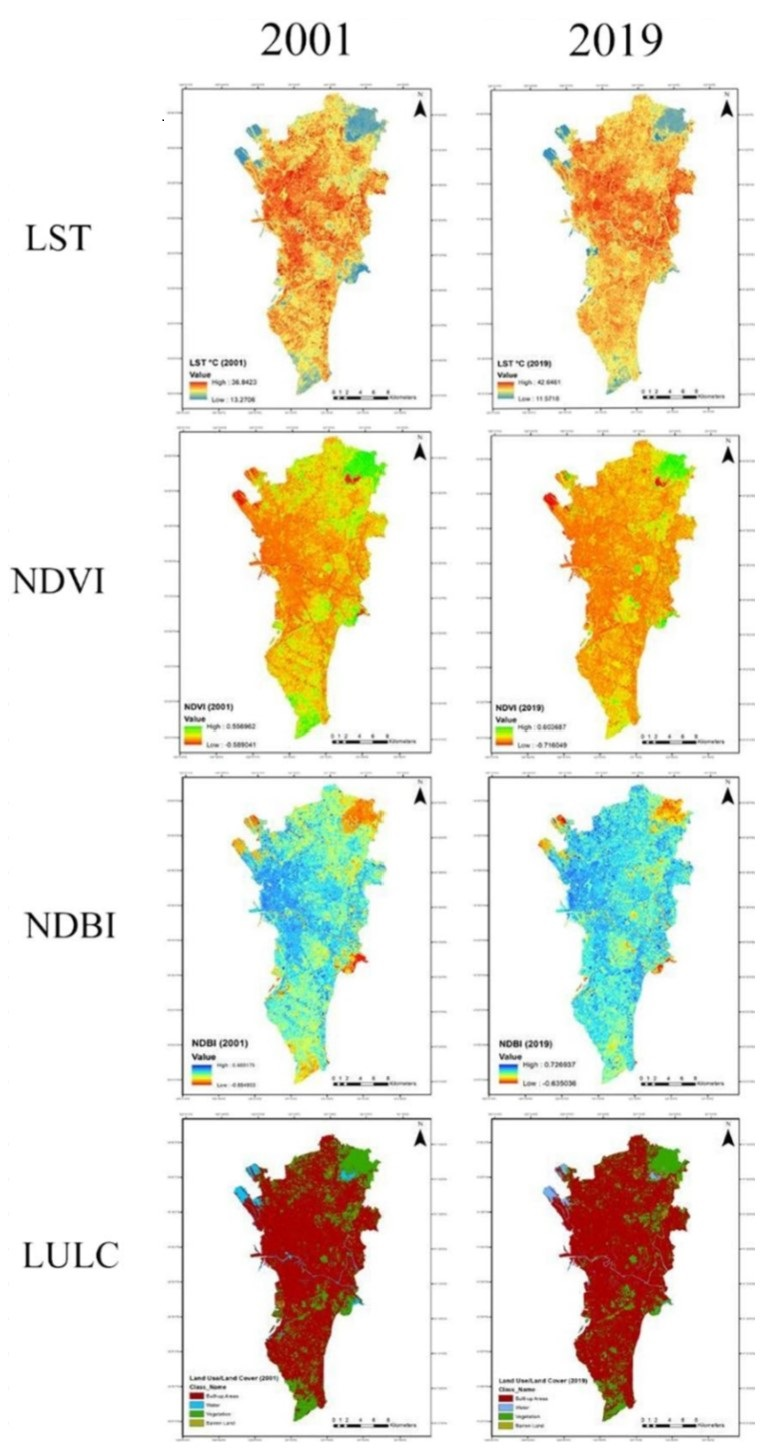
\includegraphics[height=0.9\textheight]{rrl-almadronesreyes2022-mm}
			\caption{
				The land surface temperature (LST),
				normalized difference vegetation index (NDVI), 
				normalized Difference Built-up Index (NDBI),
				and land-use/land cover (LULC)
				maps of Metro Manila in 2001 and 2019.
				Taken from \textcite{AlmadronesReyes2022}.
			}
			\label{fig:rrl-almadronesreyes2022-mm}
		\end{figure}
		
		\textcite{Purio2022} assessed the urban heat islands in Manila City using satellite and meteorological data.
		The authors report a $\qty{6}{\degreeCelsius}$ difference between the cold and hot parts of Manila.
		In addition, they note that areas with vegetation or bodies of water have lower surface temperature compared to residential areas, roadways, and commercial buildings.
		The authors have also given six recommendations the Manila city government may use in order to mitigate urban heat.
		
		\textcite{Oliveros2019} studied a total of 19 places in the Philippines with WRF to see if their urbanization efforts have had an effect on weather.
		They noted an urban heat island effect occurring, with a reported
			$\qtyrange{0.4}{2.4}{\degreeCelsius}$ minimum difference, and a 
			$\qtyrange{0.83}{2.3}{\degreeCelsius}$ maximum difference
			between urban and rural areas of Metro Manila.
		They also noted that urbanization led to more rainfall, though this finding was not statistically significant.
		
		\textcite{Cortes2022} evaluated the effectiveness of urban heat mitigation strategies in Mandaue, Cebu.
		The authors used ENVI-met, a three-dimensional software model used to simulate urban areas with computational fluid dynamics.
		They found that adding more trees and using green roofs could decrease surface temperature by about $\qtyrange{0.4}{1.1}{\degreeCelsius}$
		Notably, based on the thermal comfort index, the authors concluded that people would still feel uncomfortable from the heat, despite employing mitigation strategies.
		
		\textcite{Bilang2022} simulated the air temperature and relative humidity of Metro Manila using WRF and an urban canopy model.
		A map of their simulated heat index in Metro Manila is shown in Figure \ref{fig:rrl-bilang2022-heatindex}.
		They reported an urban heat island intensity of $\qty{8}{\degreeCelsius}$ during the daytime, and
			$\qty{3}{\degreeCelsius}$ during the nighttime.
		Places near bodies of water, such as Laguna Lake, showed lower air temperatures.
		They also showed that stagnant winds led to higher air temperatures.
		The authors remarked that it is important to use actual urban morphology values in WRF in order to get accurate results.
		
		\begin{figure}
			\centering
			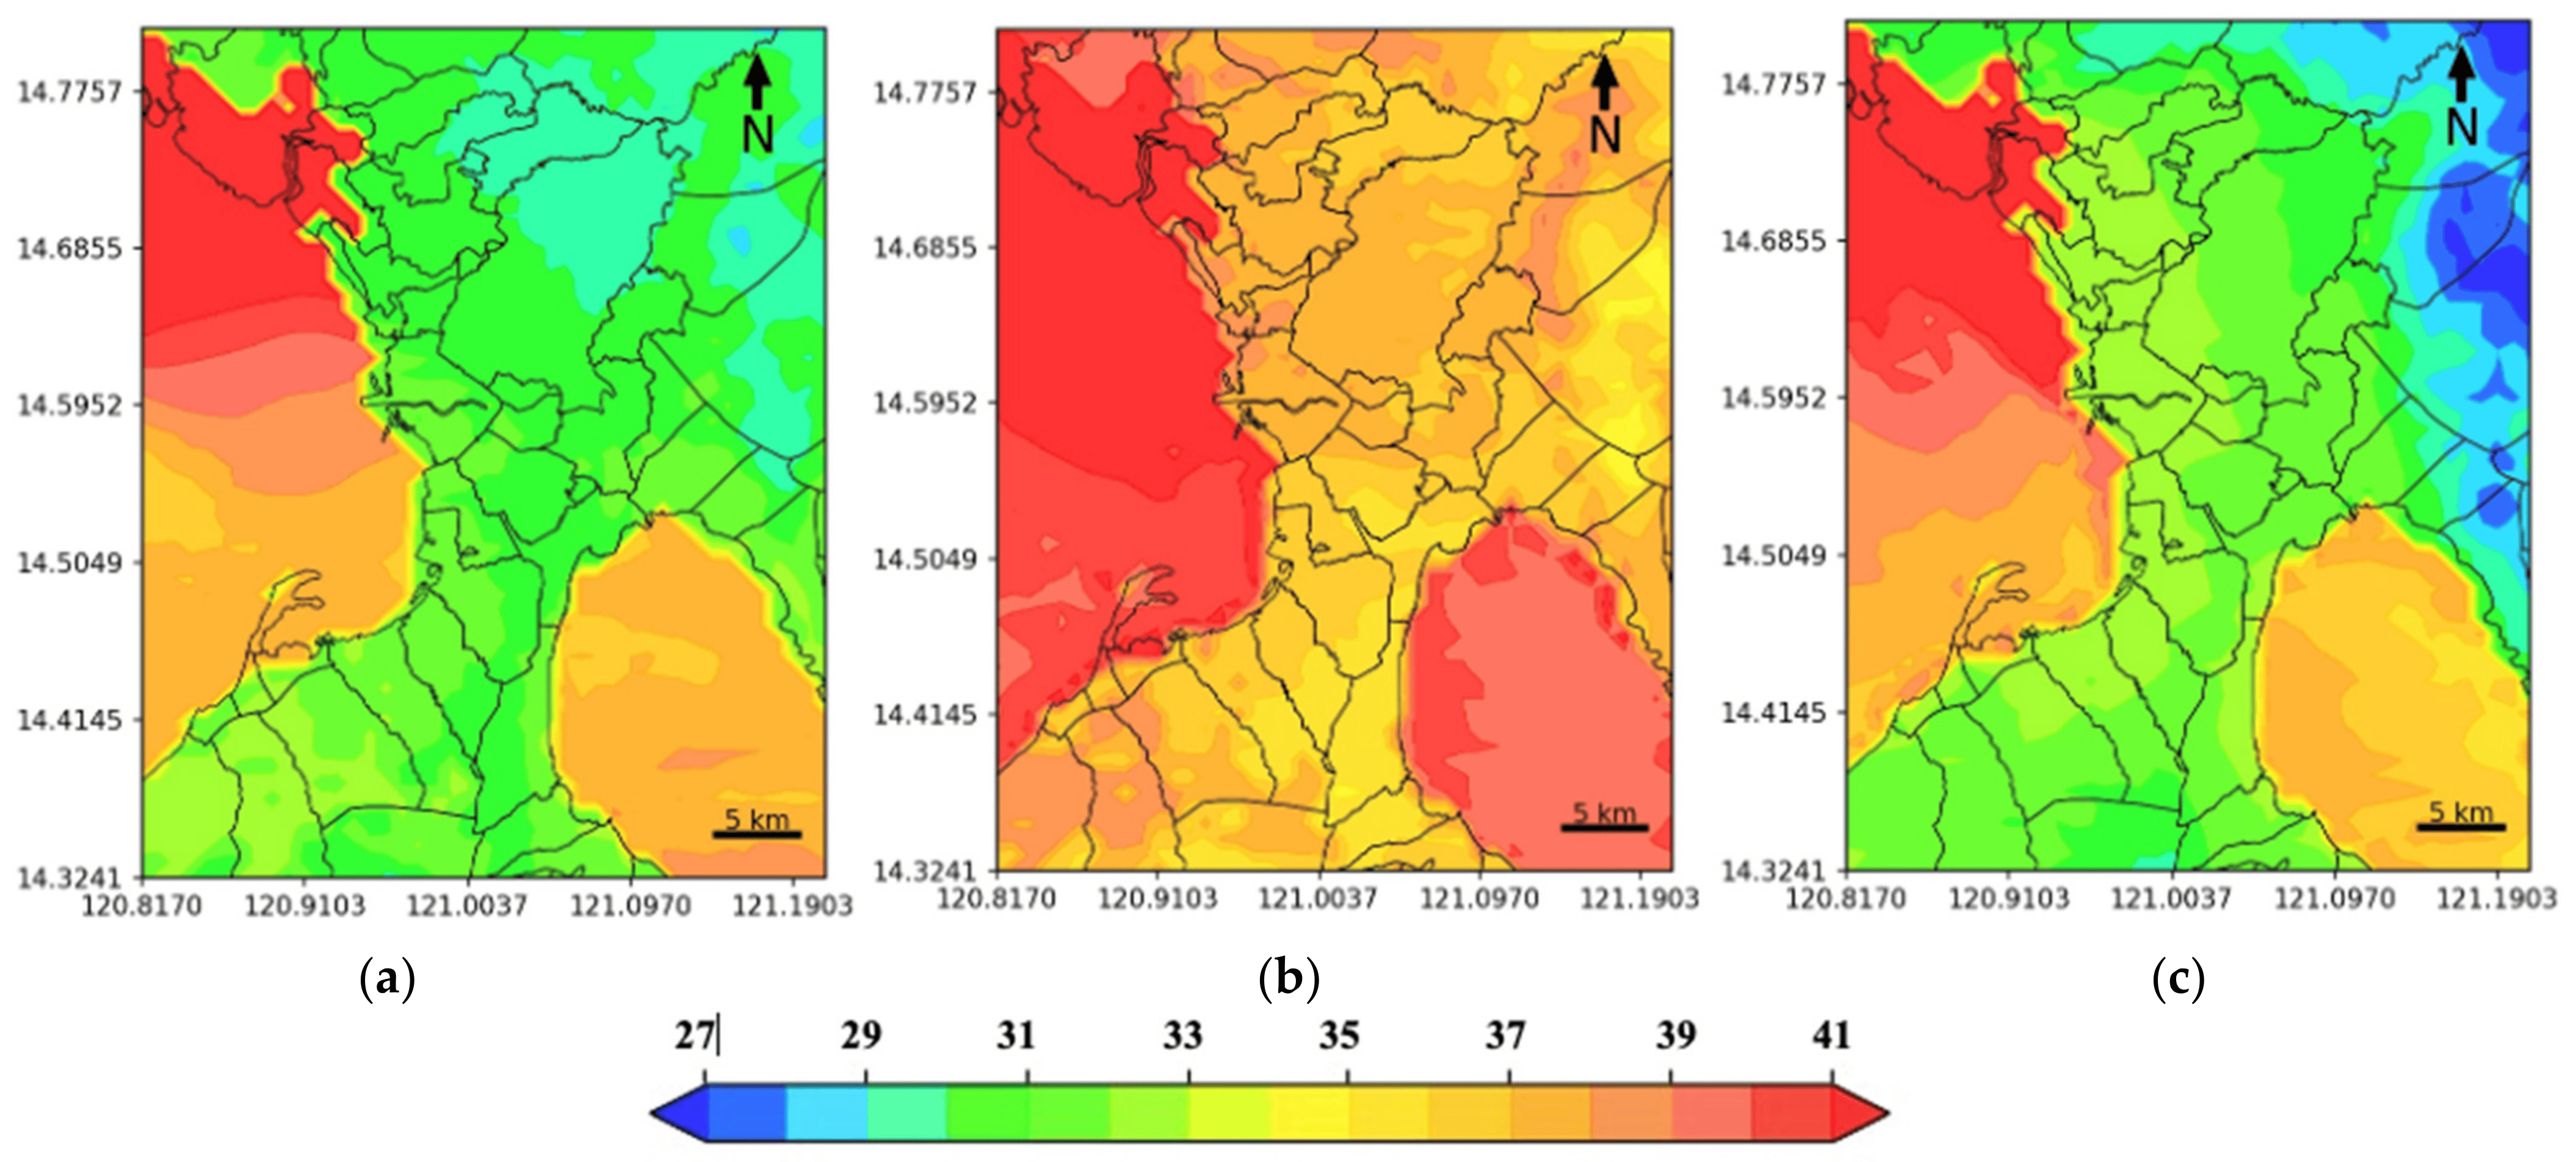
\includegraphics[width=\linewidth]{rrl-bilang2022-heatindex}
			\caption{
				Averaged heat index (\unit{\degreeCelsius}) simulated by BEM on 22–28 April 2018.
				(a) 8:00, (b) 14:00, and (c) 20:00.
				Taken from \textcite{Bilang2022}.
			}
			\label{fig:rrl-bilang2022-heatindex}
			
		\end{figure}

\section{Common Themes}
	Studies report a correlation between temperature and urbanization, which is to be expected.
	Reported temperature changes go from $\qty{1}{\degreeCelsius}$ (\cite{Huszar2018a}), 
		%up to 10 \degree C (\cite{Santamouris2020}).
		up to $\qty{8}{\degreeCelsius}$ (\cite{Wang2019}).
	For the Philippines specifically, reported temperature changes due to the urban heat island effect go from $\qty{0.4}{\degreeCelsius}$ (\cite{Oliveros2019}),
		%up to 6 \degree C (\cite{Purio2022}).
		up to $\qty{8}{\degreeCelsius}$ (\cite{Bilang2022}).
	
	There does not seem to be one common way of simulating urban heat.
	A handful of studies use the Weather Research \& Forecasting Model (WRF) with an urban canopy model.
	Other simulations include the Regional Climate Model (RegCM),
		ADMS-Urban, 
		ENVI-met, and
		the urbanized high-resolution land data assimilation system (u-HRLDAS).
	Regardless of simulation method, the studies made sure to verify their models. For example, a handful of studies compared their simulated data to data gathered via remote sensing.
	
	There have been studies that evaluate the effectiveness of urban heat mitigation strategies outside of the Philippines, such as \textcite{Gao2019} and \textcite{Gao2020}. 
	However, there is a lack of these studies inside the Philippines.
	Out of the articles mentioned in this chapter that studied the Philippines, only \textcite{Cortes2022} directly examined the effectiveness of urban heat mitigation strategies.
	\textcite{Purio2022} gives recommendations for mitigating urban heat, but studying their effectiveness was out of the authors' scope.
	
	The majority of the articles that studied the Philippines focused on Metro Manila.
	\textcite{Cortes2022} studied Mandaue, Cebu, while \textcite{Oliveros2019} studied Tagaytay, Bulacan, and fourteen other rural areas outside Metro Manila.
	
		
	%technique, results,
		%ano basehan na may urban heat problem?
		%paano sinusukat ang basehan na yun?
		%why select this location?
		%representative ba siya?
		%areas
			%materials used in buildings, its climate, what's in the area (mostly bahay? mostly trees? tubig?)
	%theory part: the physics!
		%equations
		%what simulation
	%method
		%analytical data used
	%resap2: theory. resap3: method (together with budget gant chart intro).
	%BFAR DENR DOST-SEI
	%urban heat isalands
	%yung magpappatagaL: YUNG mga runs!